\documentclass[UTF8]{ctexart}

\usepackage{ctex}
\CTEXsetup[format={\Large\bfseries}]{section}
\usepackage[top=28mm,bottom=28mm,left=15mm,right=15mm]{geometry}

\usepackage{fancyhdr}
\fancypagestyle{plain}{\pagestyle{fancy}}
\pagestyle{fancy}
\lhead{\kaishu 清华大学药学院药理毒理实验}
\newcommand{\numOfReport}[1]{\rhead{\kaishu 实验报告#1}}

\usepackage{fontspec}
\usepackage{wasysym}
\setCJKmainfont[AutoFakeBold={2}]{STZhongsong}
\setCJKmonofont{STZhongsong}

\usepackage{float}
\usepackage{booktabs}
\usepackage{tabularx}
\usepackage{array}
\usepackage{amsmath}
\usepackage{amsfonts}
\usepackage{amssymb}
\usepackage[figuresleft]{rotating}
\usepackage[para]{threeparttable}
\newcommand\info[2][40mm]{\underline{\makebox[#1][c]{#2}}}
\newcommand{\infoTable}[7]{
    \renewcommand\arraystretch{1.4}
    \begin{table}
        \begin{tabularx}{\textwidth}{
        >{\hsize=0.6\hsize\linewidth=\hsize}X
        >{\hsize=0.6\hsize\linewidth=\hsize}X
        >{\hsize=2.0\hsize\linewidth=\hsize}X
        >{\hsize=0.8\hsize\linewidth=\hsize}X
        }
            天气:\info[14mm]{#1} & 温度:\info[14mm]{#2 $^{\circ}\text{C}$} & 湿度:\info[14mm]{#3 $\%$} & 日期:#4\\
            姓名:\info[14mm]{#5} & 班级:\info[14mm]{#6} & 同组人:\info[70mm]{#7} & 
        \end{tabularx}
    \end{table}
}
\newcommand\columnC{\centering\arraybackslash}
\newcommand\columnL{\raggedright\arraybackslash}
\newcommand\columnR{\raggedleft\arraybackslash}

\usepackage{svg}
\usepackage{pdfpages}
\title{对乙酰氨基酚的镇痛作用观察}
\author{}
\numOfReport{四}

\begin{document}
\infoTable{晴}{18}{40}{10/16/2024}{何昱晖}{药3}{荣子健、马逸然、赵方一澜}
\date{}
\maketitle

\section{实验目的和原理}

\subsection{实验目的}

\begin{itemize}
    \item [(1)] 了解常用的镇痛实验方法,学习扭体法观察药物的镇痛作用的实验方法;
    \item [(2)] 用扭体法观察解热镇痛药对乙酰氨基酚的镇痛作用。
\end{itemize}

\subsection{实验原理}

在基础医学研究中筛选镇痛药的常用致痛方法有物理法(热、电、机械)和化学法。动物的疼痛反应常表现除嘶叫、舔足、翘尾、蹦跳及皮肤、肌肉抽搐。化学法,即将某些化学物质。如强酸、强碱、钾离子、缓激肽等,涂布于动物的某些敏感部位或腹腔注射。由于腹腔有广泛的感觉神经分布,某些化学物质(如冰醋酸等)注入小鼠腹腔内可刺激脏层和壁层腹膜,引起深部、大面积且持久的疼痛,致使小鼠产生扭体反应,表现为腹部两侧内凹、躯体扭曲、后肢伸展和臀部高起等行为反应,统称为「扭体反应」。本实验将 $1.2\%$ 醋酸直接腹腔注射,刺激腹膜引起持久的疼痛反应,致使小鼠出现「扭体反应」:镇痛药物可以抑制动物的「扭体反应」。本法敏感、简便、重复性好。

对乙酰氨基酚为乙酰苯胺类解热镇痛药,是一种环氧化酶抑制剂。通过选择性抑制下丘脑体温调节中枢前列腺素的合成,导致外周血管扩张、出汗而达到解热的作用:通过抑制前列腺素的合成和释放,提高痛阈而起到镇痛作用,属于外周性镇痛药。

\section{实验材料}

\begin{itemize}
    \item 实验动物:ICR 小鼠,雌雄各半,$22\sim 25\text{g}$;
    \item 药品和试剂:对乙酰氨基酚溶液、$1.2\%$ 醋酸、生理盐水等;
    \item 实验器材:注射器($1.0\text{mL}$)、天平、计时器。
\end{itemize}

\section{实验方法}

\begin{itemize}
    \item [(1)] 实验分组:各小组取 ICR 小鼠 $12$ 只,称重,编号,随机分为对照组、乙酰氨基酚低剂量组($7.5\text{mg}/\text{kg}$)、中剂量组($30\text{mg}/\text{kg}$)和高剂量组( $120\text{mg}/\text{kg}$),每组 $3$ 只小鼠;
    \item [(2)] 给药:对乙酰氨基酚低、中、高剂量组腹腔注射不同浓度的对乙酰氨基酚($0.1\text{mL}/10\text{g}$),分别为 $0.75\text{mg}/\text{mL}$、$3\text{mg}/\text{mL}$、$12\text{mg}/\text{mL}$;对照组腹腔注射等体积生理盐水($0.1\text{mL}/10\text{g}$),25 分钟后,各组小鼠分别腹腔注射 $1.2\%$ 醋酸 $75\mu\text{L}/10\text{g}$;
    \item [(3)] 镇痛作用观察:观察并记录各实验组每只小鼠首次出现「扭体反应」的时间,以及 15 分钟内小鼠出现「扭体反应」的次数。
\end{itemize}

\section{实验结果}

\begin{table}[H]
    \centering
    \begin{threeparttable}[b]
        \caption{对乙酰氨基酚的镇痛作用}
        \quad

        \begin{tabularx}{\textwidth}{
            >{\columnC\hsize=1\hsize\linewidth=\hsize}X
            >{\columnC\hsize=1\hsize\linewidth=\hsize}X
            >{\columnC\hsize=1\hsize\linewidth=\hsize}X
            >{\columnC\hsize=1\hsize\linewidth=\hsize}X
            >{\columnC\hsize=1\hsize\linewidth=\hsize}X
            >{\columnC\hsize=1\hsize\linewidth=\hsize}X
        }
            \toprule[1.5pt]
            实验分组 & 小鼠数量 & 首次出现扭体反应平均时间\tnote{1} & 平均扭体次数\tnote{2} & 镇痛百分率 & $p$ 值\\
            \midrule
            对照组 & 18 & $157.28\pm 136.12$ & $32.44\pm 13.87$ & / & /\\
            \midrule
            低剂量组 & 18 & $187.61\pm 98.61$ & $21.33\pm 12.73$ & $34.25\%$ & $0.017$\\
            \midrule
            中剂量组 & 18 & $226.17\pm 98.65$ & $25.17\pm 9.91$ & $22.43\%$ & $0.079$\\
            \midrule
            高剂量组 & 18 & $358.94\pm 233.57$ & $18.11\pm 13.96$ & $44.18\%$ & $0.004$\\
            \bottomrule[1.5pt]
        \end{tabularx}
        \begin{tablenotes}
            \item [1] 单位秒
            \item [2] 单位次/15min
        \end{tablenotes}
    \end{threeparttable}
\end{table}

\section{课后思考题}

\begin{itemize}
    \item [1] 简述常见的镇痛药分类及代表药物
    
        \begin{itemize}
            \item 阿片类:代表药物有可待因、曲马多、吗啡、羟考酮、氢吗啡酮、美沙酮、芬太尼等;
            \item 非甾体类抗炎药:代表药物有吲哚美辛、双氯芬酸、布洛芬、萘普生、洛索洛芬、尼美舒利、塞来昔布、依托考昔等;
            \item 对乙酰氨基酚;
            \item 离子通道阻滞剂:卡马西平、奥卡西平、加巴喷丁、普瑞巴林等。
        \end{itemize}

    \item [2] 简述对乙酰氨基酚的镇痛作用机制
    
        对乙酰氨基酚可能通过抑制脑内的环加氧酶-3从而减少前列腺素的合成发挥中枢止痛作用,也有研究认为该药也可以通过内源性大麻素受体提高疼痛阈值。
\end{itemize}

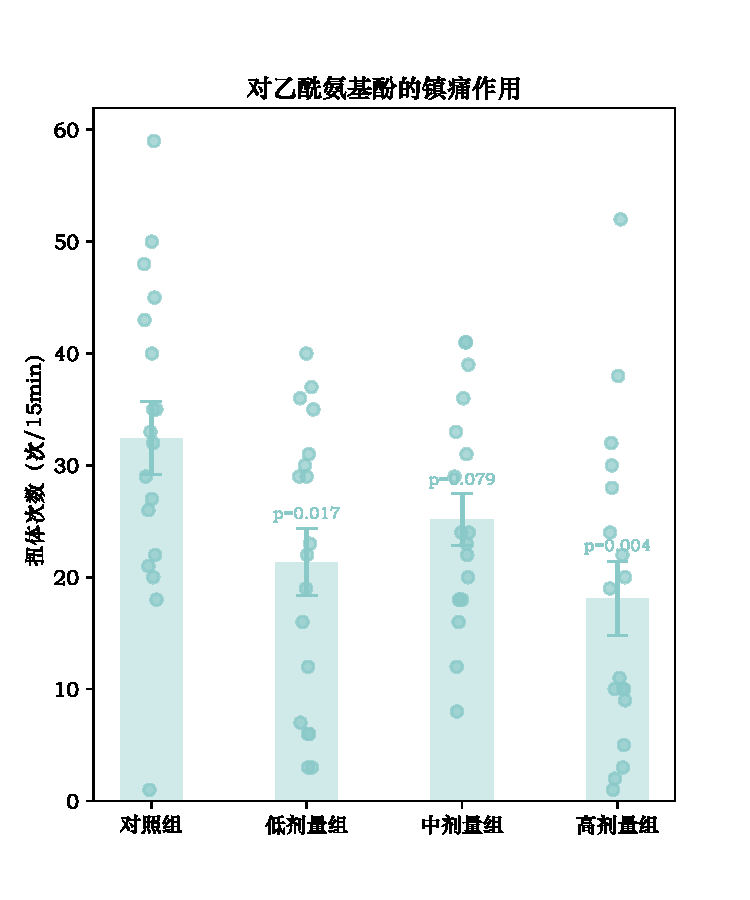
\includepdf[page={1}]{figure-4_svg.pdf}

\end{document}